
\documentclass[10pt,journal,compsoc]{IEEEtran}
\usepackage{setspace}
\usepackage{amsmath}
\usepackage{amsfonts}
\usepackage{CJK}
\usepackage{indentfirst}
%\usepackage{cite}
\usepackage{bm}
\usepackage{graphicx}
\usepackage{subfigure}
\usepackage{booktabs}
\usepackage{multirow}
\usepackage{amssymb}
\usepackage{color}
\newcommand{\red}[1]{\textcolor{red}{#1}}
\usepackage{float}
\usepackage{multicol}
\pdfminorversion=6


% *** CITATION PACKAGES ***
%
\usepackage{cite}


% *** GRAPHICS RELATED PACKAGES ***
%
\ifCLASSINFOpdf
  % \usepackage[pdftex]{graphicx}
  % declare the path(s) where your graphic files are
  % \graphicspath{{../pdf/}{../jpeg/}}
  % and their extensions so you won't have to specify these with
  % every instance of \includegraphics
  % \DeclareGraphicsExtensions{.pdf,.jpeg,.png}
\else
  % or other class option (dvipsone, dvipdf, if not using dvips). graphicx
  % will default to the driver specified in the system graphics.cfg if no
  % driver is specified.
  % \usepackage[dvips]{graphicx}
  % declare the path(s) where your graphic files are
  % \graphicspath{{../eps/}}
  % and their extensions so you won't have to specify these with
  % every instance of \includegraphics
  % \DeclareGraphicsExtensions{.eps}
\fi


% correct bad hyphenation here
\hyphenation{op-tical net-works semi-conduc-tor}


\begin{document}
%
\title{Sparsity-Aware Optimal Transport for Unsupervised Restoration Learning}

\author{Fei Wen, %, \IEEEmembership{Senior Member, IEEE},
       Wei Wang and Wenxian Yu
\IEEEcompsocitemizethanks{
	\IEEEcompsocthanksitem %Corresponding author: Fei Wen.\\  
	%This work was supported in part by the National Natural Science Foundation of China (NSFC) under Grant 62271314. 
	F. Wen, W. Wang and W. Yu are with School of Electronic Information and Electrical Engineering, Shanghai Jiao Tong University, Shanghai, China, 200240.
	E-mail: wenfei@sjtu.edu.cn; wangwei0803@sjtu.edu.cn; wxyu@sjtu.edu.cn.
}}


% The paper headers
\markboth{ }%
{Shell \MakeLowercase{\textit{et al.}}: Bare Demo of IEEEtran.cls for Computer Society Journals}


\IEEEtitleabstractindextext{%
\begin{abstract}
Recent studies show that, without any prior model, the unsupervised restoration learning problem can be optimally formulated as an optimal transport (OT) problem, which has shown promising performance on denoising tasks to approach the performance of supervised methods. However, it still significantly lags behind state-of-the-art supervised methods on complex restoration tasks such as super-resolution, deraining, and dehazing. In this paper, we exploit the sparsity of degradation in the OT framework to significantly boost its performance on these tasks. First, we disclose an observation that the degradation in these tasks is quite sparse in the frequency domain, and then propose a sparsity-aware optimal transport (SOT) criterion for unsupervised restoration learning. Further, we provide an analytic example to illustrate that exploiting the sparsity helps to reduce the ambiguity in finding an inverse map for restoration. Experiments on real-world super-resolution, deraining, and dehazing demonstrate that SOT can improve the PSNR of OT by about 2.6 dB, 2.7 dB and 1.3 dB, respectively, while achieving the best perception scores among the compared supervised and unsupervised methods. Particularly, on the three tasks, SOT significantly outperforms existing unsupervised methods and approaches the performance of state-of-the-art supervised methods.
\end{abstract}

% Note that keywords are not normally used for peerreview papers.
\begin{IEEEkeywords}
Restoration, unsupervised learning, optimal transport, super-resolution, deraining, dehazing.
\end{IEEEkeywords}}

% make the title area
\maketitle


\IEEEdisplaynontitleabstractindextext
%\IEEEpeerreviewmaketitle



%\IEEEraisesectionheading{\section{Introduction}\label{sec:introduction}}
\section{Introduction}
\label{sec:introduction}

\IEEEPARstart{I}{mage} restoration plays a fundamental 
role in low-level computer vision, which has attracted 
much research attention in the past few decades.
Traditional model based methods typically utilize 
prior models of image and/or degradation, such as
sparsity, low-rankness, smoothness, self-similarity 
or other priors of natural image, and Gaussianity, spatially 
independent i.i.d. of noise \cite{nlm,bm3d,elad1997restoration,dsc,he2010single}.
Recently, benefited from the powerful
deep learning techniques, the field of image restoration has made
much progress in the past few years \cite{mao2016image,zhang2020residual}.

Generally, the success of deep network based methods usually rely on sufficient
paired degraded-clean data. Nevertheless, in some applications
such paired data is difficult or even impractical
to collect. For such applications, as a common practice, 
synthesized degraded-clean data can be used to learn a restoration model.
However, the gap between synthesized and real-world data
limits the practical performance of the learned model on real-world data,
especially when the degradation is too complex to accurately simulate.
In these circumstances, unsupervised methods without 
requiring any degraded-clean pairs are preferred.

To relax the requirement of paired training data,
unsupervised learning methods have recently been
actively studied for various image restoration tasks.
For example, for unsupervised/self-supervised denoising
learning, the noise-to-noise (N2N) \cite{n2n}, 
noise-to-void (N2V) \cite{n2v}, noise-to-self (N2S) \cite{n2s} methods,
as well as many variants have been developed, see 
\cite{mbvd,s2s,esur,laine2019high,wu2020unpaired} and the references therein.
While N2N uses noisy pairs, N2V and N2S learn the restoration 
models in a self-supervised manner. Typically, these 
methods rely on prior assumptions, such as the noise in noisy pairs 
are independent \cite{n2n,mbvd,esur}, or the noise is spatially independent 
and/or the noise type is a priori known \cite{n2v,n2s,laine2019high,wu2020unpaired}.
Such assumptions limit the performance when the noise
does not well conform with the assumptions.

In the recent work \cite{wang2022optimal},
it has been shown that, in the absence of any 
prior model of the degradation,
the unsupervised restoration learning problem 
can be optimally formulated as an optimal transport (OT) problem.
The OT criterion based unsupervised learning method has 
achieved promising performance on various denoising 
tasks to approach the performance of supervised methods.
However, it still significantly lags behind state-of-the-art 
supervised methods on more complex restoration tasks 
such as super-resolution, deraining, and dehazing.
A main reason is that, for these restoration tasks,
seeking an inverse of the degradation map is more ambiguous.
In light of this understanding, this work is motivated to
exploit prior models of the degradation 
in the OT criterion to reduce the ambiguity in learning 
an inverse map of the degradation.

Specifically, in this work, we exploit the sparsity 
of degradation in the OT framework to significantly 
boost the performance on these complex restoration tasks. 
The main contributions are as follows.

First, we disclose an empirical observation that, for the 
super-resolution, deraining, and dehazing tasks, the degradation is 
quite sparse in the frequency domain. Based on this observation,
we propose a sparsity-aware optimal transport (SOT) criterion for 
unsupervised restoration learning. 

Then, we provide an analysis to illustrate that 
exploiting the sparsity of degradation  
in the OT criterion helps to reduce the ambiguity in finding 
an inverse map of the degradation. 

Finally, we provide extensive experimental results on both synthetic 
and real-world data for the super-resolution, deraining, 
and dehazing tasks. The results demonstrate that 
exploiting the sparsity of degradation can significantly 
boost the performance of the OT criterion.
For example, compared with the vanilla OT criterion 
on real-world super-resolution, deraining and dehazing, 
it achieves a PSNR improvement of about 2.6 dB, 2.7 dB and 1.3 dB, respectively,
and at meantime, attains the best perception scores 
among the compared supervised and unsupervised methods.
Meanwhile, in synthetic data experiments on the three tasks,
the PSNR improvement is about 2.5, 1.6, 3.4 dB, respectively.
Noteworthily, on all the tasks, SOT considerably outperforms existing unsupervised methods 
to approach the performance of state-of-the-art supervised methods.

Our work provides a generic unsupervised (unpaired) learning framework, 
which applies to various restoration applications as long as the degradation
can be sparsely represented. Relaxing the requirement 
of collecting or synthesizing paired degraded-clean data is 
of practical importance, especially for applications 
where paired data is difficult to collect or accurately simulate.
In such realistic circumstances, the proposed method has much potential
as it shows favorable performance on real-world data
even compared with state-of-the-art supervised methods.


\section{Related Work}

We review the works related to this work,
especially on unsupervised methods in various image restoration tasks.

\textbf{Image denoising}.
Traditional hand-crafted model based denoising methods 
typically design models based on a priori information on the signal and noise 
\cite{buades2005review, nlm, bm3d, lebrun2012analysis}. 
The performance of these methods is usually closely related to 
hyperparameter setting.
Recently, deep learning methods without requiring paired noisy-clean 
data have attracted active attention.
The N2N method \cite{n2n}, as well as its variants \cite{mbvd, nr2n, nac, gan2gan}, 
utilize noisy pairs to train restoration models under the assumption that
the noise is zero-mean and independent homogeneous across paired samples.
Self-supervised methods adopt special networks or training methods 
that extract information from the noisy image itself for supervised learning, 
e.g. adopting a blind-spot network to predict masked pixel by
neighboring pixels or designing sampling methods to construct paired training
data from noisy images 
\cite{n2v, n2s, s2s, neighbor2neighbor, krull2020probabilistic,laine2019high,wu2020unpaired}.
Commonly, these methods rely on the assumption that the 
noise follows independent homogeneous distribution, e.g. spatially independent.
Generally, specific prior assumptions limit realistic generalization of these methods.
More recently, based on the OT theory, the work \cite{wang2022optimal} constructs 
an optimal criterion for unpaired restoration learning in the
absence of any prior noise model. While this method has shown
promising performance that approach supervised methods on denoising 
tasks, it still significantly lags behind supervised methods on more
complex tasks such as super-resolution, deraining, and dehazing.

\textbf{Image super-resolution}. 
The research of image super-resolution has a long history 
\cite{tsai1984multiframe,elad1997restoration, schultz1996extraction, glasner2009super}.
The work \cite{dong2015image} proposes the first deep network
based super-resolution method, then deep network based super-resolution 
has attracted much attention in the past few years \cite{kim2016accurate,ledig2017photo,wang2018esrgan,ranksrgan,rcan,rnan}.
Since the method SRGAN \cite{ledig2017photo} firstly 
introduces GAN \cite{gan} into image super-resolution to improve perceptual quality, 
GAN has been widely used as a basic component in learning super-resolution 
models \cite{wang2018esrgan,ranksrgan,rcan,rnan}.
Such methods typically use synthesized paired data 
for supervised learning, e.g. by bicubic interpolation.
In order to achieve better performance on realistic data,
many unsupervised super-resolution learning methods have been developed recently. 
Most of these methods considers an unpaired setting that only unpaired low-resolution 
and high-resolution samples are available.
Basically, a mainstream of these methods are designed based on CycleGAN \cite{cyclegan}. 
To compensate for the lack of generative constraints in CycleGAN,
many improvements have been made in
\cite{lugmayr2019unsupervised, yuan2018unsupervised, usis, 
bulat2018learn, zhao2018unsupervised, wang2021unsupervised, ahn2020simusr}.

\textbf{Image deraining}. 
For image deraining, the DSC method \cite{dsc} 
uses dictionary learning as well as sparse coding,
of which the basic idea is to use a learned dictionary with strong mutual exclusion 
on a very high discriminative code that 
sparsely approximates the image blocks of both layers. 
However, its performance degrades significantly when the background of 
the input image is similar to rain drops. In the past few years,
a number of deep network based methods have 
been developed and much progress has been made
\cite{rescan,multi,wei2019semi,fu2017clearing,li2019heavy}.
Considering unsupervised methods, 
while the conditional GAN \cite{cgan} requires paired training data, 
CycleGAN \cite{cyclegan} does not and hence can be naturally employed for unsupervised 
image deraining to relax the requirement of paired data through a cyclic training structure. 
However, the generation guidance of CycleGAN is weak, 
which results in artifacts in the generated images and affects the restoration quality. 
To address this problem, DeCyGAN \cite{deraincyclegan} designs an unsupervised attention 
guided rain streak extractor to extract the rain streak masks with two constrained 
cycle-consistency branches jointly. There also exits approaches based on CycleGAN, such as \cite{jin2019unsupervised, zhu2019singe}. The work \cite{ye2022unsupervised} introduces contrastive learning into unsupervised deraining. It can separate the rain layer from clean image with the help of the intrinsic self-similarity property within
samples and the mutually exclusive property between the two layers.

\textbf{Image dehazing}. 
Image dehazing has long been a challeging problem \cite{fattal2008single}, 
for which the dark channel prior (DCP) based method \cite{he2010single} 
is a classic model-based method. In \cite{he2010single}, it is observed that
in most non-sky patches of clean images, there exists at least one color channel 
has very low intensity at some pixels, and in comparison, 
local patches of hazy images tend to have a greater brightness (less dark).
Recently, the work \cite{golts2019unsupervised} only uses hazy images for 
model training by minimizing a DCP loss. 
In addition to the supervised methods 
\cite{cai2016dehazenet,aodnet,dehamer,gcanet,ffanet},
many unsupervised methods, which learn the dehazing map from 
unpaired clean and hazy images, have been developed recently.
For example, the works \cite{yang2018towards, zhao2021refinednet} use GAN 
to extract the information of clean images from hazy ones. 
As CycleGAN is a typical unsupervised framework, many methods 
improve on it with specific designs 
\cite{dudhane2019cdnet, engin2018cycle, zhao2019dd, liu2020end}.
Moreover, the D4 method \cite{d4} explored the scattering coefficients and 
depth information contained in hazy and clean images. By estimating 
the scene depth, it is able to re-render hazy images with different 
thicknesses, which further facilitates the training of the dehazing network.


\section{Preliminaries}

This section first presents the problem formulation 
and then introduces the OT based unsupervised 
restoration learning method.

\subsection{Problem Formulation}

Consider a degradation to restoration process as
\[X~\longrightarrow ~Y ~\stackrel{f}{\longrightarrow} ~\hat{X},\]
where $X \sim {p_X}$ is the source, 
$Y$ is the degraded observation,
$\hat X: = f(Y)$ is the restoration with $f$
being the restoration model to be learned.
Meanwhile, without loss of generality, 
we consider a typical additive model for 
the degradation as
\begin{equation}
Y = X + N,
\label{eq_degradation}
\end{equation}
where $N$ stands for the degradation.

Note that among the three restoration tasks considered 
in this work, while the degradation models 
for the deraining and dehazing tasks
directly conform to this additive model,
it is not the case for the super-resolution task as it
involves resolution reduction from $X$ to $Y$.
However, model (\ref{eq_degradation}) still applies
when we consider the frequency domain model, since  
resolution reduction is in fact equivalent to a loss of 
high-frequency components in the frequency domain.
As will be presented in Section 4, 
the proposed method uses a fidelity loss in frequency domain.

Generally, due to the information loss in the data 
process chain $X\rightarrow Y$,
seeking an inverse process from $Y$ to $X$ for 
restoration is ambiguous and suffers from distortion.
The ideal goal of restoration 
is to seek an inverse process with the lowest distortion.
It is to suppress/remove/rectify the degradation in the 
observation $Y$ as much as possible, and at meantime, 
preserve the information of the source $X$ contained in $Y$ as much as possible.
Besides, for some image restoration tasks,
high perception quality is another objective in addition to low distortion,
which reflects the degree to which the restoration $\hat X$ looks like 
a valid natural clean sample from human’s perception.

Accordingly, an optimal criterion to fulfill the above goals,
e.g., degradation suppression, maximally information preserving of $X$, 
and high perception quality, is given by
\begin{equation}
\begin{array}{c}
\mathop {\max }\limits_f I\left( {f(Y);X} \right)\\
{\rm{subject \ to \ }}~~d({p_{\hat X}},{p_{ X}}) \le 0,
\end{array}
\label{eq_optimal_supervised}
\end{equation}
where $I(\cdot;\cdot)$ is the mutual information.
$d(\cdot,\cdot)$ is a divergence measures 
the deviation between two distributions, 
such as the Kullback-Leibler divergence or Wasserstein distance, 
which satisfies $d(p, q) \geq 0$ and 
$d(p, q) = 0\Leftrightarrow {p = q}$ for any distributions $p$ and $q$. 
The perceptual quality of restoration is measured by the distribution 
divergence from natural samples as $d({p_{\hat X}},{p_{ X}})$.
It has been well recognized that perception quality
is associated with the deviation from natural sample statistics \cite{wang2006quality,mittal2012no,moorthy2011blind,SaadBC12 }. The constraint $d({p_{\hat X}},{p_{ X}}) \le 0$ enforces
${p_{\hat X}}={p_X}$, which ensure the restoration having perfect perception quality.
It has been recently revealed that 
%high perception quality can only be achieved
%at some cost of restoration distortion that %\cite{blau2018perception,yan2021perceptual}.
pursuing high perception quality would inevitably 
lead to increase of the lowest 
achievable distortion \cite{blau2018perception,yan2021perceptual,blau2019rethinking, yan2022perceptual}.
To implement criterion (\ref{eq_optimal_supervised}),
degraded-clean pairs $\{(Y,X)\}$ are required for supervision.
%This criterion maximizes the mutual information 
%between the reconstruction $f(Y)$ and the ground-truth 
%$X$ while constraining the reconstruction to have 
%the same distribution as natural clean images.


\subsection{OT for Unsupervised Restoration Learning}

OT can be traced back to the seminal work of 
Monge \cite{monge1781memoire} in 1781, 
with significant advancements by Kantorovich 
\cite{kantorovich1942translation} in 1942. 
It has a well-established theoretical foundation 
and provides a powerful framework for comparing 
probability measures based on their underlying geometry.
OT has recently received increasing attention in machine learning \cite{kolouri2017optimal,Villani2003,wgan}.

Computationally, the OT problem seeks the most efficient transport map of transforming one distribution of mass to another with minimum cost.
Specifically, let ${\cal P}(X)$ and ${\cal P}(Y)$ denote two sets of probability measures on $X$ and $Y$, respectively. 
Meanwhile, let $\nu  \sim {\cal P}(Y)$ and $\mu \sim {\cal P}(X)$ denote two probability measures.
The OT problem seeks the most efficient transport plan from $\nu $ to $\mu$ that minimizes the transport cost.

\textbf{Definition 1. (Transport map)}: 
Given two probability measures $\nu \sim {\cal P}(Y)$ 
and $\mu  \sim {\cal P}(X)$,
$f:Y \to X$ is a transport map from $\nu$ to $\mu$ if
\begin{equation}
\mu (A) = \nu ({f^{ - 1}}(A)) \nonumber,
\end{equation}
for all $\mu$-measurable sets $A$.

\textbf{Definition 2. (Monge’s optimal transport problem) \cite{monge1781memoire}}: 
For a probability measure $\nu$, let ${f_{\sharp}} \nu$ denote the transport of $\nu$ by $f$.
Let $c:Y \times X \to [0, + \infty ]$ be a cost function that $c(y,x)$ measures the cost of transporting $y \in Y$ to $x \in X$. Then, given two probability measures $\nu \sim {\cal P}(Y)$ and $\mu \sim {\cal P}(X)$, the OT problem is defined as%find a $\nu$-measurable map $f:Y \to X$ by
\begin{equation}
\begin{array}{c}
\mathop {\inf }\limits_f \int_Y {c\left( {f(y),y} \right)} d\nu (y)\\
{\rm{subject \ to\ }}~~\mu  = {f_\# }\nu ,
\end{array}
\label{eq_MongeOT}
\end{equation}
over $\nu$-measurable maps $f:Y \to X$.
A minimum to this problem, e.g. denoted by ${f^*}$, 
is called an OT map from $\nu$ to $\mu$.

The OT problem seeks a transport plan to turn the mass of 
$\nu $ into $\mu $ at the minimal geometric cost measured 
by the cost function $c$, e.g. typically 
$c\left( {f(y),y}\right): = {\left\|{f(y)-y} \right\|^\beta}$ with $\beta\ge 1$.

In the absence of any degraded-clean pairs for supervised 
learning of the restoration model, an unsupervised learning
method using only unpaired noisy and clean data has been 
proposed in \cite{wang2022optimal} based on the OT 
formulation (\ref{eq_MongeOT}) as
\begin{equation}
\begin{gathered}
  \mathop {\min }\limits_f {\mathbb{E}_{Y \sim {p_Y}}}\left(\left\|Y-f(Y)\right\|^\beta\right) \\
  {\text{subject \ to \ }}~~{p_{\hat X}} = {p_X}.
\end{gathered}
\label{eq_ot}
\end{equation}

Formulation (\ref{eq_ot}) is an OT problem seeks a 
restoration map $f$ from $Y$ to $X$. 
The constraint ${p_{\hat X}} = {p_X}$ enforces 
that the restoration $\{\hat X\}$ 
has the same distribution as natural clean images $\{X\}$.
Under this constraint, the restoration would have good perception quality, 
i.e. looks like natural clean images, since each $\hat X$
lies in the manifold (set) of $X$ \cite{blau2018perception,yan2021perceptual,blau2019rethinking, yan2022perceptual}.
Meanwhile, the constraint ${p_{\hat X}} = {p_X}$
imposes an image prior stronger than any hand-crafted priors,
such as sparsity, low-rankness, smoothness and dark-channel prior.
These priors have been widely used in traditional 
image restoration methods. Any reasonable prior model
for natural clean images would be fulfilled under 
the constraint ${p_{\hat X}} = {p_X}$.

The objective in \eqref{eq_ot} imposes fidelity 
of the restoration $\hat X$ to $Y$, 
which ensures minimum distance transport and hence
the restoration map can maximally preserve the 
information of $X$ contained in $Y$ \cite{wang2022optimal}.
From the data process chain $X\rightarrow Y \rightarrow\hat{X}$, 
it follows that $I(\hat X;X) \leq I(Y;X)$. 
Hence, under the constraint on $\hat{X}$, maximally preserving the information of $X$ contained in $Y$
in the restoration can be fulfilled by maximizing the mutual 
information $I(\hat X;Y)$. 

In contrast, when without the fidelity term, 
formulation \eqref{eq_ot} can be implemented by standard GAN
to generate $\hat X$ satisfies ${p_{\hat X}} = {p_X}$, e.g,
by $\mathop {\min }\limits_f d({p_X},{p_{\hat X}})$.
However, the map from $Y$ to $X$ is no longer an 
minimum distance transport and the restoration $\hat X$
may be excessively far from the clean source $X$.
For instance, the generator $f$ can disregard the input $Y$ 
and randomly generate samples $\hat{X}$ from the distribution ${p_X}$ 
to satisfy ${{p_{\hat X}} = p_X}$ but with $\hat{X}$ 
be independent on $X$, i.e., $I(\hat{X};X)=0$.
The conditional GAN \cite{cgan} does not suffer from
this degeneration problem by discriminating between $(Y,X)$ and $(Y,\hat X)$, 
but requires paired degraded-clean data $(Y,X)$ for supervision. 
RoCGAN \cite{RoCGAN} also uses paired degraded-clean data.
Although AmbientGAN does not require paired degraded-clean, 
it requires a pre-defined degradation model 
which can be easily sampled \cite{ambientgan}. 
Similarly, NR-GAN \cite{nrgan} does not suffer
from such limitation, but requires either 
known noise distribution type or noise satisfying some
invariant properties. 

In implementation, the OT based formulation \eqref{eq_ot} 
is relaxed into an unconstrained form as
\begin{equation}
\mathop {\min }\limits_f {{\mathbb E}_{Y \sim {p_Y}}}\left(\left\|Y-f(Y)\right\|^\beta\right) + \lambda d({p_X},{p_{\hat X}}),
\label{eq_ot_unconstrained}
\end{equation}
where $\lambda > 0$ is a balance parameter. 
%$d(\cdot,\cdot)$ is a divergence measures the deviation between two distributions, such as the Kullback-Leibler divergence or Wasserstein distance, 
%which satisfies $d(p, q) \geq 0$ and $d(p, q) = 0\Leftrightarrow {p = q}$ for any distributions $p$ and $q$. 
Then, formulation (\ref{eq_ot_unconstrained})
is implemented based on WGAN-gp \cite{wgangp}.
Though relaxed, it has been shown in 
\cite{wang2022optimal} that under certain 
conditions the unconstrained formulation 
(\ref{eq_ot_unconstrained}) has the same 
solution as the original constrained 
formulation (\ref{eq_ot}) in theory.
However, in practice the balance parameter $\lambda$
needs to be tuned to achieve satisfactory performance.
More recently, an OT algorithm for
unpaired super-resolution has been
proposed in \cite{ot-sr2022}, which is 
an alternative for solving (\ref{eq_ot}).

%for unpaired SR which learns an unbiased OT map for the perceptual transport cost.


\section{Incorporating Sparsity Prior into 
OT for Unsupervised Restoration Learning}

The degradation map $X\rightarrow Y$ in (1) is typically non-injective and
inevitably incurs information loss of the source $X$.
Hence, the degradation map is non-invertible and seeking
an inverse of it is ambiguous. In this scenario, exploiting
prior information of the degradation map is an effective way
to reduce the inverse ambiguity. In this section, we first
show the sparsity property of the degradation for three
representative restoration tasks, and then exploit this property
in the OT framework to propose a sparsity-aware
formulation for restoration learning. Furthermore, we provide an analytic
example to show the effectiveness of exploiting sparsity in
reducing the ambiguity of inverting the degradation process.

\subsection{The Sparsity of Degradation}

\begin{figure*}[!t]
	\centering
	\subfigure[Super-resolution]
         {
		\includegraphics[width=0.3\linewidth]{fre_sr.png}
	  }
         \subfigure[Deraining]
         {
		\includegraphics[width=0.3\linewidth]{fre_rain.png}
	}
         \subfigure[Dehazing]{
		\includegraphics[width=0.3\linewidth]{fre_fog.png}
	}
	\caption{Histograms of the degradation $N$ in the frequency domain for three restoration tasks. (a) Super-resolution (500 real-world images from the RealVSR dataset \cite{realVSR}). (b) Deraining (400 real-world images from the SPA dataset \cite{spa}). (c) Dehazing (200 real-world images from the Dense-haze dataset \cite{dense}). The degradation in the three tasks are very sparse in the frequency domain, which follows a hyper Laplacian distribution.}
	\label{fig_sparse}
\end{figure*}

In what follows, we show that for three representative restoration tasks,
super-resolution, deraining, and dehazing, the degradation $N$ is very sparse
in the frequency domain. Fig. 1 presents the histogram statistic of the
degradation in the frequency domain for each of the three tasks.
500 real-world images from the super-resolution dataset RealVSR \cite{realVSR},
400 real-world images from the deraining dataset SPA \cite{spa}, and 200
real-world images from the dehazing dataset Dense-haze \cite{dense} are used to
compute the histogram statistic for the three tasks, respectively.
Given $L$ degraded-clean pairs $\{(y_i,x_i)\}_{i=1,\cdots,L}$ from a dataset,
%the histogram in the pixel domain is computed based on the absolute amplitude of the degradation  , whilst
the histogram in the frequency domain is computed based on
the absolute FFT coefficients $\{|{\rm{fft2}}(y_i-x_i)|\}_{i=1,\cdots,L}$,
${\rm{fft2}}(\cdot)$ is the 2D FFT. Each histogram is averaged over the image
pair number $L$. For super-resolution, $Y$ is obtained from a $1/4$ times
low resolution version of $X$ by 4 times bicubic up-sampling.

It can be seen from Fig. 1 that, for each of the three tasks,
the frequency domain representation of the degradation is very sparse,
which follows a hyper-Laplacian distribution.
%Meanwhile, the FFT representation of the degradation follows a distribution that is much sparser than that of the pixel domain representation.
This significant sparsity feature of the degradation provides
a natural and useful prior for restoration inference.
It is exploited in our method by promoting sparsity of the
degradation in the frequency domain %in restoration learning
to achieve more accurate restoration.
Note that although these statistic results are derived based on
real-world degradation data, the implementation of our algorithm
does not require an accurate estimation of the sparsity parameter
of the degradation and, as will be shown in experiments,
a rough selection of $q$ of the $\ell_q$ cost
(e.g. $q\in\{0.5,1\}$) is enough for achieving satisfactory performance.

\subsection{Proposed Method Exploiting Degradation Sparsity in OT}

The optimal transport criterion (\ref{eq_ot}) does not impose any
constraint on the degradation $N$. Though optimal in the case without prior information of the degradation, it is suboptimal when
prior information of the degradation is available. For example,
if the distribution of $N$ is \textit{a priori} known, an ideal
criterion extending (\ref{eq_ot}) becomes
\begin{equation}
\begin{gathered}
  \mathop {\min }\limits_f {\mathbb{E}_{Y \sim {p_Y}}}\left(\left\|f(Y)-Y\right\|^\beta\right) \\
  {\text{subject \ to \ }}~~{p_{\hat X}} = {p_X},~{p_{\hat N}} = {p_N},
\end{gathered}
\label{eq_ot_knowPn}
\end{equation}
where $N:=Y-f(Y)=Y-\hat{X}$. Adding the constraint ${p_{\hat N}} = {p_N}$
can effectively leverage the prior information of the degradation process (\ref{eq_degradation})
to find a better transport map for the inverse problem $Y\rightarrow X$ with
lower distortion. While the distribution $p_X$ can be learned from natural
clean images, seeking an estimation of $p_N$ requires the collection of
sufficient degradation $\{n_i\}$. In fact, if a collection of sufficient
degradation $\{n_i\}$ is available, degraded-clean pairs $\{x_j+n_i,x_j\}$
can be directly obtained and the restoration model can be learned in a
supervised manner. However, in practice, collecting real-world degradation
$\{n_i\}$ would be as difficult as collecting real-world degraded-clean pairs $\{(y_i,x_i)\}$.

In this work, we relax the requirement of $p_N$ and employ a simple
generic prior for the degradation instead. It is inspired by the above empirical
observation that for some restoration tasks the degradation is very sparse
in the frequency domain, as shown in Fig. \ref{fig_sparse}. Specifically, we propose
a formulation to make use of the frequency domain sparsity of degradation as
\begin{equation}
\begin{gathered}
  \mathop {\min }\limits_f {\mathbb{E}_{Y \sim {p_Y}}}\left(\left\|\mathcal{F}(f(Y)-Y)\right\|^q_q\right) \\
  {\text{subject \ to \ }}~~{p_{\hat X}} = {p_X},
\end{gathered}
\label{eq_sot}
\end{equation}
where $\mathcal{F}(\cdot)$ stands for the discrete Fourier transform,
and $\|\cdot\|^q_q$ is the $\ell_q$-norm with $0\leq q\leq 1$.
Since the FFT representation of $N$, i.e. $\mathcal{F}(N)$, is sparse,
a necessary condition for an inverting map $f$ to be optimal is that
it should conform to this property such that $\mathcal{F}(N)=\mathcal{F}(f(Y)-Y)$ is sparse.
To achieve this, in formulation (\ref{eq_sot}) we use the $\ell_q$-norm
loss with $0\leq q\leq 1$ to promote the sparsity. The $\ell_q$-norm
is a sparsity-promotion loss in data fitting, which has been widely used
in sparse recovery to obtain sparse solution \cite{lq,wen2016robust}.

For the particular case of $q=2$, formulation (\ref{eq_sot}) reduces
to the OT problem (\ref{eq_ot}) with $\ell_2$ cost since
$\|\mathcal{F}(f(Y)-Y)\|^2_2=\|f(Y)-Y\|^2_2$.
The $\ell_2$ cost is optimal for degradation with Gaussian distribution
but not optimal for sparse degradation with super-Gaussian distribution.
As it has been shown in Fig. 1 that, the frequency domain distribution
of degradation is far from Gaussian rather being hyper-Laplace, using
$\ell_2$ cost can result in unsatisfactory performance far from optimal.

In implementation, an unconstrained form of (\ref{eq_sot}) is used as
\begin{equation}
  \mathop {\min }\limits_f {\mathbb{E}_{Y \sim {p_Y}}}\left(\left\|\mathcal{F}(f(Y)-Y)\right\|^q_q\right) +
  \lambda d(p_{\hat X}, p_X),
\label{eq_sot_unconstrained}
\end{equation}
where $\lambda>0$ is a balance parameter.
As the discrete Fourier transform is complex-valued, for a vector $M\in\mathbb{C}^{m+1}$, the $\ell_q$ loss is computed as
\begin{equation}
\|M\|_q^q=\sum_{i=0}^m\left(\Re^2\{M(i)\}+\Im^2\{M(i)\}\right)^{\frac{q}{2}}.
\label{eq_comlex_lq}
\end{equation}

\subsection{An Analysis on the Effectiveness of the Sparsity Prior}

%Due to the intrinsic structures in natural images,
%it is usually assumed that natural images lie in a
%%low-dimensional manifold in the high-dimensional pixel space.
Under the degradation process $Y=X+N$, the distribution of $Y$
is a convolution of the distributions of $X$ and $N$,
i.e., $p_Y=p_X\otimes p_N$. Generally, the inverse problem
from $Y$ to $X$ is ambiguous due to the information loss
in the degradation process. In the absence of any prior
information of $N$, the optimal transport map $f_{\sharp}p_Y=p_X$ obtained
by (\ref{eq_ot}) can be used as an ideal inverse (restoration) map \cite{wang2022optimal}.
However, when prior information of $N$ is available, the map $f$ is
no longer optimal and does not necessarily approach the lower bound
of inverse distortion. Naturally, the prior information of $N$ can be
exploited to reduce the inverting ambiguity to some extent and hence
result in lower restoration distortion.

As our objective is to exploit the underlying sparsity of $N$ to reduce
the inverse ambiguity, here we use an example to show the effectiveness
of exploiting the sparsity of the degradation in helping to find the
desired correct inverse map.

\textbf{Example 1 [Exploiting the sparsity of degradation helps to
find an inverse map with lower distortion].}
Consider a discrete random source $X\in \mathbb{R}^{m+1}$,
which follows a two-point distribution with probability mass function as
\begin{equation}\notag
p_X(x) = \left\{\! {\begin{array}{*{20}{l}}
\!{p_1,}&{x=x_1}\\
\!{p_2,}&{x=x_2}
\end{array}} \right.,
\end{equation}
with
\[x_1=[-a,\mathop{\underbrace{b,\cdots,b}}\limits_{m}]^T,~~~~x_2=[-a,\mathop{\underbrace{-b,\cdots,-b}}\limits_{m}]^T,\]
where $a\gg b>0$ such that $a^2>mb^2$ and $a^q<mb^q$ for any $0\leq q\leq 1$.
For example, these two conditions hold for $a=1$, $b=0.1$ and $10<m<100$.
If only considering $q=0$, they hold for $a=1$, $b=0.1$ and $1<m<100$.
Furthermore, consider a degradation process as (\ref{eq_degradation}),
where $N\in \mathbb{R}^{m+1}$ also follows a two-point distribution
with probability mass function given by
\begin{equation}\notag
p_N(n) = \left\{\! {\begin{array}{*{20}{l}}
\!{\tilde{p}_1,}&{n=n_1}\\
\!{\tilde{p}_2,}&{n=n_2}
\end{array}} \right.,
\end{equation}
with
\[n_1=[-2a,0,\cdots,0]^T,~~~~n_2=[2a,0,\cdots,0]^T.\]
Note that $N$ is sparse as only one of its elements is nonzero.
In this setting, the distribution of $Y$ is given by the convolution
between $p_X$ and $p_N$ as
\begin{equation}\notag
p_Y(y) = \left\{\! {\begin{array}{*{20}{l}}
\!{p_1\tilde{p}_1,}&{y=y_1}\\
\!{p_1\tilde{p}_2,}&{y=y_2}\\
\!{p_2\tilde{p}_1,}&{y=y_3}\\
\!{p_2\tilde{p}_2,}&{y=y_4}
\end{array}} \right.,
\end{equation}
with
\[y_1=[-3a,b,\cdots,b]^T,~~~~y_2=[a,b,\cdots,b]^T,\]
\[y_3=[-a,-b,\cdots,-b]^T,~~~~y_4=[3a,-b,\cdots,-b]^T.\]

Then, given the distributions of $X$ and $Y$, we investigate
the inverse process $Y\rightarrow X$ by seeking the OT
from $p_Y$ to $p_X$ with different cost functions.
Particularly, we evaluate the $\ell_q$ cost with $0\leq q \leq 1$
in comparison with the widely used $\ell_2$ cost.

First, with the $\ell_2$ cost and under the condition $a^2>mb^2$,
a solution $f_2^*:Y\rightarrow X$ to the OT problem
\begin{equation}
\begin{gathered}
  \mathop {\min }\limits_{f_2} {\mathbb{E}_{Y \sim {p_Y}}}\left(\left\|f_2(Y)-Y\right\|^2_2\right) \\
  {\text{subject \ to \ }}~~(f_2)_{\sharp}{p_Y} = {p_X},
\end{gathered}
\label{eq_sot_examp_f2}
\end{equation}
would map $y_2\rightarrow x_2$ rather than $y_2\rightarrow x_1$ since
$\|y_2-x_2\|^2_2=4mb^2<\|y_3-x_2\|^2_2=4a^2$ and $y_3\rightarrow x_1$
rather than $y_3\rightarrow x_2$ since $\|y_3-x_1\|^2_2=4mb^2<\|y_3-x_2\|^2_2=4a^2$.
For example, let $p_1=\tilde{p}_1=0.5$ and $p_2=\tilde{p}_2=0.5$,
the optimal map $f_2^*$ is given by $f_2^*(y_1)=x_1$, $f_2^*(y_2)=x_2$,
$f_2^*(y_3)=x_1$, and $f_2^*(y_4)=x_2$, as illustrated in Fig. \ref{fig_example}(b).
In contrast, with the $\ell_{q}$ cost and under the condition $a^q<mb^q$, $\forall q\in[0,1]$,
it follows that $\|y_2-x_2\|^q_q=m(2b)^q>\|y_3-x_2\|^q_q=(2a)^q$.
Hence, the solution $f_q^*:Y\rightarrow X$ to the OT problem
\begin{equation}
\begin{gathered}
  \mathop {\min }\limits_{f_q} {\mathbb{E}_{Y \sim {p_Y}}}\left(\left\|f_q(Y)-Y\right\|^q_q\right) \\
  {\text{subject \ to \ }}~~(f_q)_{\sharp}{p_Y} = {p_X},
\end{gathered}
\label{eq_sot_examp_fq}
\end{equation}
is given by $f_q^*(y_1)=x_1$, $f_q^*(y_2)=x_1$ and
$f_q^*(y_3)=x_2$, $f_q^*(y_4)=x_2$, 
as illustrated in Fig. \ref{fig_example}(c).

\begin{figure}[!t]
	\centering
	\subfigure[Degradation process]
         {
		\includegraphics[width=0.28\linewidth]{fig_example_a.png}
	  }~~~~
         \subfigure[Inverse via OT with $\ell_2$ cost]
         {
		\includegraphics[width=0.28\linewidth]{fig_example_b.png}
	}~~~~
         \subfigure[Inverse via OT with $\ell_q$ cost for any $0\leq q \leq 1$]{
		\includegraphics[width=0.28\linewidth]{fig_example_c.png}
	}
	\caption{An illustration of the optimal transport from $p_Y$ to
$p_X$ with different cost function in Example 1. (a) The degradation process $Y=X+N$. (b) Inverse via the optimal transport $f_2$ with $\ell_2$ cost. (c) Inverse via the optimal transport $f_q$ with $\ell_q$ cost for any $0\leq q \leq 1$. In this example, the optimal transport map under the $\ell_q$ cost yields the correct inverse map with zero distortion, while that under the $\ell_2$ cost does not.}
	\label{fig_example}
\end{figure}

In this example, the residual $N$ is very sparse as it has only
one nonzero element. This sparsity property can be exploited by
using a sparsity-promotion data fitting cost, such as the $\ell_q$-norm
with $0\leq q \leq 1$ \cite{lq,wen2016robust}. Since using the $\ell_q$ cost
can well exploit the underlying sparsity prior of the degradation
to reduce the ambiguity in finding the inverse map, in this example
it yields the desired correct inverse map under the OT criterion,
which has a zero distortion. In comparison, the $\ell_2$ cost yields
an undesired map, which does not align with the degradation map and
has a nonzero distortion, as shown in Fig. 2.  This example illustrates
that exploiting the sparsity prior of the degradation (e.g., by the
$\ell_q$ cost) can effectively help to find an inverse transport map
with lower restoration distortion.

\section{Experimental Results}

We conduct experimental evaluation on three image restoration tasks, 
including super-resolution, deraining, and dehazing. For each task, 
the proposed method is compared with state-of-the-art supervised and 
unsupervised methods on both synthetic and real-world data.
Note that, since for each of the tasks there exists a number of
supervised and unsupervised methods, it is difficult to compare with 
all the representative methods in each task. The focus here is to 
compare with state-of-the-art supervised and unsupervised methods
in each task. Particularly, state-of-the-art supervised
methods are used as ideal baselines for comparison.
For our method, two variants, denoted by SOT ($\ell_{0.5}$) and SOT ($\ell_1$), 
are evaluated in each task, which use the $\ell_{0.5}$ cost and $\ell_{1}$ cost, respectively.
The compared methods are as follows.

\begin{itemize}
\item[$\bullet$]
For the super-resolution task, the compared supervised methods 
include RankSR \cite{ranksrgan}, RCAN \cite{rcan}, 
ESRGAN \cite{wang2018esrgan} and RNAN \cite{rnan}. 
The compared unsupervised methods include USIS \cite{usis}, 
OT\cite{wang2022optimal}.%, SOT ($\ell_{0.5}$) and SOT ($\ell_1$), 
%where SOT ($\ell_{0.5}$) and SOT ($\ell_1$) are two variants of 
%our method use the $\ell_{0.5}$ and $\ell_{1}$ cost, respectively.
\vspace{3pt}\item[$\bullet$]
For the deraining task, the compared methods 
include DSC\cite{dsc}, RESCAN\cite{rescan}, 
MPRNet\cite{multi}, SIRR\cite{wei2019semi}, 
CycleGAN\cite{cyclegan}, DeCyGAN\cite{ deraincyclegan}, 
OT\cite{wang2022optimal}, where DSC is a traditional method, 
RESCAN and MPRNet are supervised methods, SIRR is a semi-supervised method, 
while CycleGAN, DeCycleGAN and OT are unsupervised methods.
\vspace{3pt}\item[$\bullet$]
For the dehazing task, the compared methods include DCP \cite{he2010single}, 
AODNet \cite{aodnet}, Dehamer \cite{dehamer}, GCANet \cite{gcanet}, 
FFANet \cite{ffanet}, D4 \cite{ d4}, OT \cite{wang2022optimal}, 
where DCP is a traditional model-based method, 
AODNet, Dehamer, GCANet and FFANet are supervised learning methods, 
wile D4 and OT are unsupervised learning methods. 
\end{itemize}

In order to make a comprehensive evaluation, the restoration quality
is evaluated in terms of both distortion metrics, 
including peak signal to  noise  ratio  (PSNR) and structural similarity (SSIM),
and perceptual quality metrics, including perception index (PI) \cite{pi} and 
learned perceptual image patch similarity (LPIPS) \cite{lpips}.

We implement the proposed formulation (\ref{eq_sot_unconstrained}) based on 
WGAN-gp \cite{wgangp}, with $0 \leq q \leq 1$ and $\lambda $ being tuned for 
each task. Note that the best selection of the value of $q$ depends on 
the statistics of the data and hence is application and data dependent.
In practice it is generally difficult to select the optimal value of $q$.
Therefore, in the implementation we only roughly test two values of $q$, 
e.g., $q=0.5$ and $q=1$ for the $\ell_q$ cost of SOT.
Experimental results show that this rough selection is 
sufficient to yield satisfactory performance of SOT.
%Although accurate estimation of the sparsity parameter of the residuals can effectively improve the reconstruction, these statistic results are derived based on real-world degradation data. So in the implementation, only the parameters $q=0.5$ and $q=1$ are roughly chosen to construct the $\ell_q$ loss, and the experiments verify that this approach is sufficient to achieve satisfactory reconstruction results.

For a fair comparison, our method and the OT method \cite{wang2022optimal}
use the same network structure, which consists of a generator and a discriminator. 
The generator uses the network in MPRNet \cite{multi}, which is one of the state-of-the-art models, 
while the discriminator is the same as that in \cite{wang2022optimal}. 
The discriminator takes the generator output (restored images) and clean images as input. 
It should be noted that although clean images are used here, 
the proposed method is unsupervised because the noisy input of 
the generator (restoration model) and the clean images 
input to the discriminator are not paired.

\subsection{Synthetic Image Super-Resolution}

First, we conduct super-resolution experiment 
on synthetic data. The used DIV2K\cite{div2k} 
dataset contains a total of 1000 high-quality RGB 
images with a resolution of about 2K. 100 images are 
used for testing. Since OT requires the input to have 
the same size as the output, we follow the pre-upsampling 
method \cite{wang2020deep} to upsample the low-resolution 
images before feeding them into the network by bicubic.
%The bicubic upsampled images are used as a benchmark 
%to compare against supervised and unsupervised methods.


\begin{table}[!t]
	\renewcommand\arraystretch{2}
	\footnotesize
	\centering
	\caption{Quantitative comparison on 4x super-resolution of synthetic images (using the DIV2K dataset).}
        \begin{tabular}{|cc|c|c|}
		\hline
		\multicolumn{2}{|c|}{\textbf{Method}}                               & \textbf{PSNR/SSIM} & \textbf{LPIPS/PI}            \\ \hline
		\multicolumn{1}{|c|}{\textbf{Traditional}}                   & Bicubic & 26.77/0.755 & 0.1674/7.07 \\ \hline
		\multicolumn{1}{|c|}{\multirow{4}{*}{\textbf{Supervised}}}  & RankSR\cite{ranksrgan}  & 26.56/0.734 & 0.0541/\textbf{3.01} \\ \cline{2-4} 
		\multicolumn{1}{|c|}{}                       & RCAN\cite{rcan}    & \textbf{29.33}/\textbf{0.828} & 0.0925/5.24 \\ \cline{2-4} 
		\multicolumn{1}{|c|}{}                       & ESRGAN\cite{wang2018esrgan}  & 26.66/0.749 & \textbf{0.0520}/3.26 \\ \cline{2-4} 
		\multicolumn{1}{|c|}{}                       & RNAN\cite{rnan}    & 29.31/0.827 & 0.0966/5.40 \\ \hline
		\multicolumn{1}{|c|}{\multirow{4}{*}{\textbf{Unsupervised}}} & USIS\cite{usis}    & 22.22/0.628 & 0.1761/3.52 \\ \cline{2-4} 
		\multicolumn{1}{|c|}{}                       & OT\cite{wang2022optimal}     & 25.73/0.719 & 0.0838/4.44 \\ \cline{2-4} 
		\multicolumn{1}{|c|}{}                       & SOT ($\ell_{0.5}$)   & 28.25/0.801 & 0.0612/3.03 \\ \cline{2-4} 
		\multicolumn{1}{|c|}{}                       & SOT ($\ell_1$)  & 27.91/0.783 & 0.0821/3.45 \\ \hline
	\end{tabular}
\end{table}

\begin{figure}[!t]
	\centering
	\includegraphics[width=0.86\linewidth] {PSNR_lambda.png}
	\caption{Restoration PSNR of SOT in image super-resolution for different values of $\lambda$.}
	\label{figure2}
\end{figure}

\begin{figure*}[!t]
	\centering
	\subfigure[Test image]{
		\includegraphics[width=0.3\linewidth]{DIV2K_valid_HR.png}
	}\subfigure[Ground truth]{
		\includegraphics[width=0.3\linewidth]{DIV2K_valid_HR2.png}
	}\subfigure[Bicubic (26.59 dB)]{
		\includegraphics[width=0.3\linewidth]{bicubic.png}
	}
	\subfigure[RankSR (26.64/0.743/0.053)]{
		\includegraphics[width=0.3\linewidth]{RankSR.png}
	}\subfigure[RCAN (\textbf{29.35}/\textbf{0.829}/0.093)]{
		\includegraphics[width=0.3\linewidth]{RCAN.png}
	}\subfigure[ESRGAN (26.66/0.751/\textbf{0.052})]{
		\includegraphics[width=0.3\linewidth]{ESRGAN.png}
	}
	\subfigure[USIS (23.44/0.701/0.167)]{
		\includegraphics[width=0.3\linewidth]{USIS.png}
	}\subfigure[OT (26.88/0.754/0.082)]{
		\includegraphics[width=0.3\linewidth]{results_pre_ot_100.png}
	}\subfigure[SOT ($\ell_{0.5}$) (28.62/0.821/0.060)]{
		\includegraphics[width=0.3\linewidth]{results_pre.png}
	}
	\caption{Visual comparison on 4x synthetic image super-resolution. The PSNR/SSIM/LPIPS results are provided in the brackets. The images are enlarged for clarity.}
	\label{figure1}
\end{figure*}


Table 1 presents quantitative results of 4x super-resolution 
on the DIV2K dataset. It can be seen that the proposed method SOT
can achieve PSNR and SSIM results close to those of state-of-the-art 
supervised learning methods, e.g., with about 1.06 dB difference 
compared with RCAN. Meanwhile, in terms of the perception indices,
its perceptual quality exceeds some of the supervised methods 
such as RCAN. It should be noted that both RankSR and ESRGAN
take perceptual quality as the reconstruction target and 
use perceptual quality metrics such as LPIPS as the optimization 
target during training. Hence, they can achieve 
better perceptual quality scores. 
However, recent studies on the trade-off between distortion and 
perceptual quality show that, the improvement in perceptual quality 
would necessarily lead to increase of reconstruction distortion, 
e.g. the deterioration of the MSE, PSNR and SSIM metrics 
\cite{blau2019rethinking,yan2021perceptual}. Accordingly, 
the PSNR and SSIM results of RankSR and ESRGAN are worse. 
Moreover, by exploiting the degradation sparsity,
the proposed SOT significantly outperforms the
vanilla OT method, e.g. an improvement of about 2.52 dB in PSNR. 
Using the $\ell_{0.5}$ cost yields better results of SOT than the
$\ell_{1}$ cost.

%Moreover, if we compare the methods based on optimal transport, we find that introducing residual sparsity can greatly improve the reconstruction quality. Besides, $SOT(\ell_{0.5})$ performs better than $SOT(\ell_{1})$, which may be due to the fact that the distribution of its residuals in the frequency domain is closer to the $\ell_{0.5}$ curve.

Fig. \ref{figure2} shows the PSNR of SOT versus the value of $\lambda$,
which investigates the effect of the parameter $\lambda$. 
Fig. \ref{figure1} compares the visual quality of 4x 
super-resolution on a typical sample from the DIV2K dataset. 
It can be seen that the result of RCAN, which yields the
highest PSNR, is closer to the ground-truth, but the 
reconstructed images appear to be blurred and the 
details are not clear enough. 
The proposed SOT method with the $\ell_{0.5}$ cost yields higher PSNR
than RankSR and ESRGAN, while having comparable perception quality.

%While the methods with 
%higher LPIPS scores can yield clearer texture, 
%they tend to introduce texture artifacts. 
%The proposed SOT($\ell_{0.5}$) method can achieve reconstruction results close to the ground truth while retaining clearer image texture information, which significantly improves the image reconstruction quality.
%It can be found that the value of $lambda$ will have a significant effect on the  reconstruction quality, which is contrary to the theoretical analysis, probably because WGAN-gp can only approximate the W-distance between distributions.

\subsection{Real-Word Image Super-Resolution}

\begin{table}[!t]
	\renewcommand\arraystretch{2}
	\footnotesize
	\centering
	\caption{Quantitative comparison on real-world image super-resolution (using the RealVSR dataset).}
        \begin{tabular}{|cc|c|c|}
		\hline
		\multicolumn{2}{|c|}{\textbf{Method}}                               & \textbf{PSNR/SSIM} & \textbf{LPIPS/PI}           \\ \hline
		\multicolumn{1}{|c|}{\textbf{Traditional}}                   & Bicubic & 23.15/0.749 & 0.1347/5.94
		 \\ \hline
		\multicolumn{1}{|c|}{\multirow{4}{*}{\textbf{Supervised}}}  & RankSR\cite{ranksrgan}  & 21.05/0.607 & 0.1031/\textbf{2.79} \\ \cline{2-4} 
		\multicolumn{1}{|c|}{}                       & RCAN\cite{rcan}    & 23.39/0.772 & 0.1573/5.79 \\ \cline{2-4} 
		\multicolumn{1}{|c|}{}                       & ESRGAN\cite{wang2018esrgan}  & 21.13/0.632 & 0.1024/3.53 \\ \cline{2-4} 
		\multicolumn{1}{|c|}{}                       & RNAN\cite{rnan}    & 23.19/0.752 & 0.1599/5.88 \\ \hline
		\multicolumn{1}{|c|}{\multirow{4}{*}{\textbf{Unsupervised}}} & USIS\cite{usis}    & 19.06/0.502 & 0.2122/3.35 \\ \cline{2-4} 
		\multicolumn{1}{|c|}{}                       & OT\cite{wang2022optimal}     & 21.34/0.658 & 0.1110/4.12 \\ \cline{2-4} 
		\multicolumn{1}{|c|}{}                       & SOT ($\ell_{0.5}$)   & \textbf{23.89}/\textbf{0.782} & 0.0839/3.27 \\ \cline{2-4} 
		\multicolumn{1}{|c|}{}                       & SOT ($\ell_1$)  & 22.85/0.722 & \textbf{0.0758}/3.23 \\ \hline
	\end{tabular}
\end{table}

In synthetic super-resolution experiments, bicubic down-sampling 
is widely used to construct paired training data. However, 
real-word degradation can substantially deviate from bicubic down-sampling.
This limits the performance of the synthetic data learned model on real-world data.
To further verify the performance of the proposed method on real scenes, 
we conduct experiment on a real-world super-resolution dataset RealVSR \cite{realVSR}. 
In this dataset, paired data is constructed by firstly using the 
multi-camera system of iPhone 11 Pro Max to capture images 
of different resolutions in the same scene separately, 
and then adopting post-processing such as color correction and pixel alignment. 
The results on this dataset are shown in Table 2.

\begin{figure*}[!t]
	\centering
	\subfigure[Test image]{
		\includegraphics[width=0.32\linewidth]{test_gt_sr.png}
	}\subfigure[Ground truth]{
		\includegraphics[width=0.32\linewidth]{test_gt_sr2.png}
	}\subfigure[bicubic (23.01 dB)]{
		\includegraphics[width=0.32\linewidth]{test_sr.png}
	}
	\subfigure[RankSR (20.87/0.612/0.104)]{
		\includegraphics[width=0.32\linewidth]{RankSR_sr.png}
	}\subfigure[RCAN (23.48/0.784/0.157)]{
		\includegraphics[width=0.32\linewidth]{RCAN_sr.png}
	}\subfigure[ESRGAN (21.06/0.634/0.101)]{
		\includegraphics[width=0.32\linewidth]{ESRGAN_sr.png}
	}
	\subfigure[USIS (19.57/0.527/0.211)]{
		\includegraphics[width=0.32\linewidth]{USIS_sr.png}
	}\subfigure[OT (21.65/0.674/0.111)]{
		\includegraphics[width=0.32\linewidth]{results_real2_sr.png}
	}\subfigure[SOT ($\ell_{0.5}$) (\textbf{24.03}/\textbf{0.792}/\textbf{0.084})]{
		\includegraphics[width=0.32\linewidth]{results_real_sr.png}
	}
	\caption{Visual comparison on real-world image super-resolution. The PSNR/SSIM/LPIPS results are provided in the brackets. The images are enlarged for clarity.}
	\label{figure3}
\end{figure*}


From the results, the proposed method can achieve better 
PSNR, SSIM and LPIPS scores even compared with state-of-the-art 
supervised methods. Moreover, exploiting degradation sparsity 
can improve the performance of the OT method by a large margin.
For example, SOT($\ell_{0.5}$) achieves a PSNR about 2.55 dB higher than OT
with significant better perception scores.
%reconstruction quality since SOT gets higher scores than OT. 
SOT($\ell_{0.5}$) has lower distortion than SOT($\ell_{1}$) 
(e.g. about 1 dB higher in PSNR) but with worse perception scores.
This  accords well with the distortion-perception tradeoff theory.

Fig. \ref{figure3} compares the visual quality of the 
methods on a typical sample from the RealVSR dataset. 
It can be seen that SOT achieves the best 
PSNR, SSIM and LPIPS scores. Qualitatively, 
it can achieve high-quality detail reconstruction
while having less artifacts than the perception-oriented methods.

\subsection{Synthetic Image Deraining}

For synthetic image deraining, we train the models on 
the Rain1800 dataset \cite{zhang2019image} and test on 
the Rain100L dataset \cite{yang2017deep}. These two datasets 
respectively contain 1800 and 100 images of natural scenes 
with simulated raindrops.

\begin{table}[!t]
	\renewcommand\arraystretch{2}
	\footnotesize
	\centering
	\caption{Quantitative comparison of the deraining methods on synthetic data 
 (the Rain1800 and Rain100L datasets are used for training and testing, respectively).}
        \begin{tabular}{|cc|c|c|c|}
		\hline
		\multicolumn{2}{|c|}{\textbf{method}}                                                       & \textbf{PSNR/SSIM}   & \textbf{LPIPS/PI}     \\ \hline
		\multicolumn{1}{|c|}{\textbf{}}                        & Rainy                           & 25.52/0.825                        & 0.1088/3.77                       \\ \hline
		\multicolumn{1}{|c|}{\textbf{Traditional}}                    & DSC\cite{dsc}                            & 25.72/0.831                       & 0.1116/2.79                       \\ \hline
		\multicolumn{1}{|c|}{}                                 & RESCAN\cite{rescan}                         & 29.80/0.881                        & 0.0731/2.87                        \\ \cline{2-4} 
		\multicolumn{1}{|c|}{\multirow{-2}{*}{\textbf{Supervised}}}  & MPRNet\cite{multi}                         & \textbf{36.40}/\textbf{0.965}                        & 0.0167/3.21                      \\ \hline
		\multicolumn{1}{|c|}{\textbf{Semi-supervised}}                   & SIRR\cite{wei2019semi}                           & 23.48/0.800                        & 0.0978/2.88                        \\ \hline
		\multicolumn{1}{|c|}{}                                 & CycleGAN\cite{cyclegan}                       & 24.03/0.820                        & 0.0960/2.80                       \\ \cline{2-4} 
		\multicolumn{1}{|c|}{}                                 & DeCyGAN\cite{deraincyclegan}                 & 24.89/0.821                        & 0.0952/3.12                        \\ \cline{2-4} 
		\multicolumn{1}{|c|}{}                                 & OT\cite{wang2022optimal}                             & 33.71/0.954                        & 0.0158/2.76                        \\ \cline{2-4} 
		\multicolumn{1}{|c|}{}                                 & SOT ($\ell_{0.5}$)                           & 34.74/0.948                        & 0.0132/2.54                       \\ \cline{2-4} 
		\multicolumn{1}{|c|}{\multirow{-5}{*}{\textbf{Unsupervised}}}  &SOT ($\ell_{1}$) &  35.33/0.963 & \textbf{0.0108}/\textbf{2.51} \\ \hline
	\end{tabular}
\end{table}

Table 3 shows the quantitative results tested on the Rain100 dataset. 
Clearly, the proposed method can achieve a PSNR close to the state-of-the-art 
supervised method. For example, the difference in PSNR between SOT($\ell_{1}$) 
and MPRNet is about 1.07 dB. Noteworthily, SOT($\ell_{1}$) 
achieves the best perception scores among all the compared unsupervised 
and supervised methods.
%the perceptual quality even surpasses supervised methods. 
Again, SOT performs much better than OT, which demonstrates the 
effectiveness sparsity exploitation. For SOT, the $\ell_{1}$ cost
yields better performance than the $\ell_{0.5}$ cost.

\begin{figure*}[!t]
	\centering
	\subfigure[Test image]{
		\includegraphics[width=0.3\linewidth]{test_gt.png}
	}\subfigure[Ground truth]{
		\includegraphics[width=0.3\linewidth]{test_gt2.png}
	}\subfigure[Rainy (25.41 dB)]{
		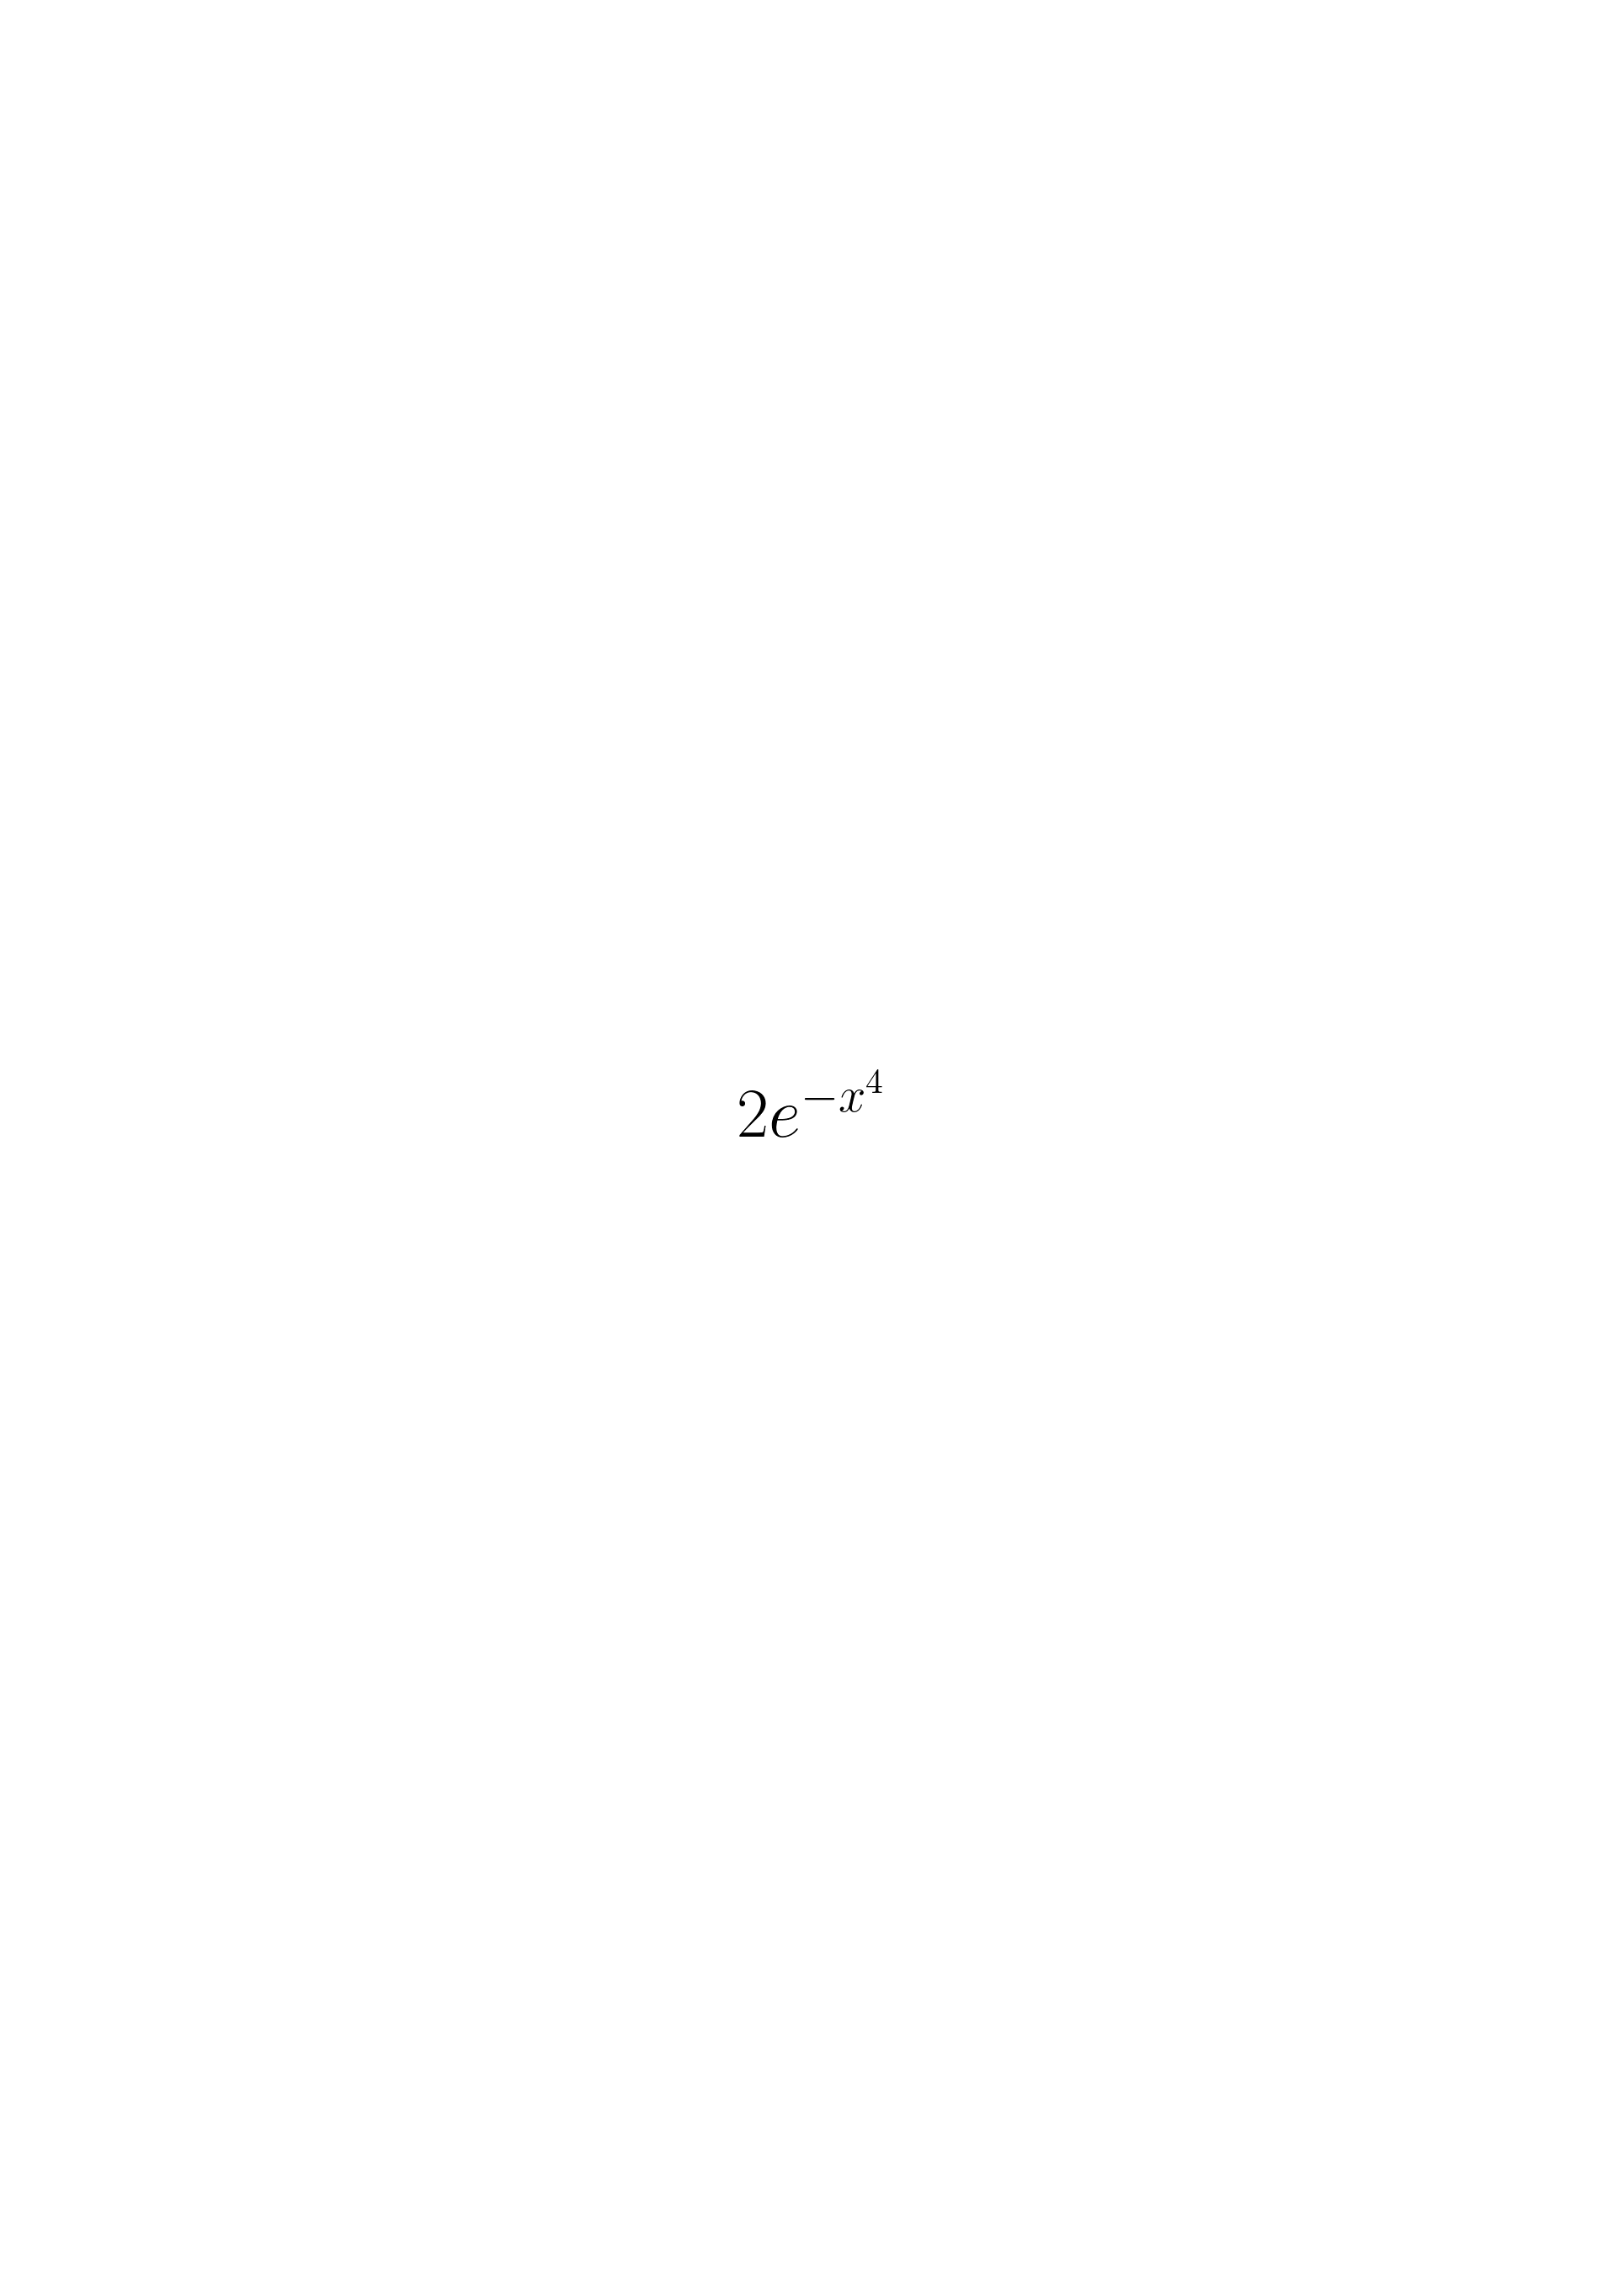
\includegraphics[width=0.3\linewidth]{test.png}
	}
	\subfigure[DSC (25.78/0.835/0.112)]{
		\includegraphics[width=0.3\linewidth]{dsc.png}
	}\subfigure[RESCAN (30.21/0.892/0.072)]{
		\includegraphics[width=0.3\linewidth]{RESCAN.png}
	}\subfigure[MPRNet (\textbf{36.58}/\textbf{0.972}/0.018)]{
		\includegraphics[width=0.3\linewidth]{MPRNet.png}
	}
	\subfigure[SIRR (24.59/0.825/0.098)]{
		\includegraphics[width=0.3\linewidth]{SIRR.png}
	}\subfigure[DeCyGAN (25.32/0.865/0.095)]{
		\includegraphics[width=0.3\linewidth]{DeCycleGAN.png}
	}\subfigure[SOT ($\ell_{1}$) (36.02/0.968/\textbf{0.011})]{
		\includegraphics[width=0.3\linewidth]{ot1.png}
	}
	\caption{Visual comparison on synthetic image deraining. The PSNR/SSIM/LPIPS results are provided in the brackets. The images are enlarged for clarity.}
	\label{figure4}
\end{figure*}

Fig. \ref{figure4} compares the visual quality of the methods.
It can be observed that the supervised methods, such as MPRNet, 
can achieve excellent rain removal but with the restoration being over-smoothing.
The proposed method can reconstruct better texture details, 
while achieving effective rain removal.

\begin{table}[!t]
	\renewcommand\arraystretch{2}
	\footnotesize
	\centering
	\caption{Quantitative comparison of the deraining methods on real-world data (using the SPA dataset  \cite{spa}).}
        \begin{tabular}{|cc|c|c|c|}
		\hline
		\multicolumn{2}{|c|}{\textbf{method}}                                                       & \textbf{PSNR/SSIM}   & \textbf{LPIPS/PI}     \\ \hline
		\multicolumn{1}{|c|}{\textbf{}}                        & Rainy                           & 34.30/0.923                        & 0.0473/8.49                      \\ \hline
		\multicolumn{1}{|c|}{\textbf{Traditional}}                    & DSC\cite{dsc}                            & 32.29/0.921                      & 0.0498/7.89                       \\ \hline
		\multicolumn{1}{|c|}{}                                 & RESCAN\cite{rescan}                         & 38.34/0.961                        & 0.0250/8.03                        \\ \cline{2-4} 
		\multicolumn{1}{|c|}{\multirow{-2}{*}{\textbf{Supervised}}}  & MPRNet\cite{multi}                         & \textbf{46.12}/\textbf{0.986}                        & 0.0109/7.68                      \\ \hline
		\multicolumn{1}{|c|}{\textbf{Semi-supervised}}                   & SIRR\cite{wei2019semi}                           & 22.66/0.710                        & 0.1323/7.87                        \\ \hline
		\multicolumn{1}{|c|}{}                                 & CycleGAN\cite{cyclegan}                       & 28.79/0.923                        & 0.0422/7.58                       \\ \cline{2-4} 
		\multicolumn{1}{|c|}{}                                 & DeCyGAN\cite{deraincyclegan}                 & 34.78/0.929                        & 0.0528/7.50                        \\ \cline{2-4} 
		\multicolumn{1}{|c|}{}                                 & OT\cite{wang2022optimal}                             & 41.68/0.951                        & 0.0098/7.35                        \\ \cline{2-4} 
		\multicolumn{1}{|c|}{}                                 & SOT ($\ell_{0.5}$)                           & 42.69/0.958                        & 0.0096/7.15                       \\ \cline{2-4} 
		\multicolumn{1}{|c|}{\multirow{-5}{*}{\textbf{Unsupervised}}}  &SOT ($\ell_{1}$) &  44.37/0.982 & \textbf{0.0084}/\textbf{7.06} \\ \hline
	\end{tabular}
\end{table}


\subsection{Real-world Image Deraining}

For the real-world image derainging experiment, 
we chose the real scene dataset SPA \cite{spa} for training and testing. 
This dataset takes images with and without rain in the same scene by 
fixing the camera position, hence the rain-free images can be used as 
the ground-truth for supervised model training. The experimental results 
are shown in Table 4.

Similar to the results in the synthetic deraining experiment,
the proposed method achieves the best performance among the unsupervised methods. 
It achieves a PSNR only 1.75 dB lower than  
the state-of-the-art supervised method MPRNet.
Particularly, SOT achieves the best perception scores, 
which even surpasses that of the supervised methods.
In addition, SOT($\ell_1$) attains a PSNR 2.69 dB higher than
that of the vanilla OT method.

\begin{figure*}[!t]
	\centering
	\subfigure[Ground truth]{
		\includegraphics[width=0.3\linewidth,height=0.2\linewidth]{test_gt_r.png}
	}\subfigure[Rainy (35.26 dB)]{
		\includegraphics[width=0.3\linewidth,height=0.2\linewidth]{test_r.png}
	}\subfigure[DSC (32.36/0.915/0.050)]{
		\includegraphics[width=0.3\linewidth,height=0.2\linewidth]{dsc_r.png}
	}
	\subfigure[RESCAN (38.65/0.962/0.024)]{
		\includegraphics[width=0.3\linewidth,height=0.2\linewidth]{RESCAN_r.png}
	}\subfigure[MPRNet (45.62/\textbf{0.982}/0.011)]{
		\includegraphics[width=0.3\linewidth,height=0.2\linewidth]{MPRNet_r.png}
	}\subfigure[SIRR (22.31/0.689/0.132)]{
		\includegraphics[width=0.3\linewidth,height=0.2\linewidth]{SIRR_r.png}
	}
	\subfigure[CycleGAN (30.27/0.856/0.040)]{
		\includegraphics[width=0.3\linewidth,height=0.2\linewidth]{cycleGAN_r.png}
	}\subfigure[DeCyGAN (34.58/0.918/0.053)]{
		\includegraphics[width=0.3\linewidth,height=0.2\linewidth]{DeCycleGAN_r.png}
	}\subfigure[SOT ($\ell_{1}$) (\textbf{45.72}/0.979/\textbf{0.008})]{
		\includegraphics[width=0.3\linewidth,height=0.2\linewidth]{result_ot_full_r.png}
	}
	\caption{Visual comparison on real-world image deraining. The PSNR/SSIM/LPIPS results are provided in the brackets. }
	\label{figure5}
\end{figure*}

Fig. \ref{figure5} compares the visual quality of 
the deraining methods on a typical real sample. 
It can be seen that, SOT can achieve a quality 
on par with the state-of-the-art supervised method MPRNet
to provide a visually plausible restoration, which
demonstrate the effectiveness of SOT on real data.
It should be noted that although CycleGAN can also achieve 
excellent rain removal, it introduces additional distortion such as color, 
resulting in larger distortion, e.g., with a PSNR more 
than 10 dB lower than that of MPRNet and SOT.
%even achieves higher PSNR and LPIPS scores than the state-of-the-art supervised method MPRNet. 

\subsection{Synthetic Image Dehazing}

Hazy scenes, like rainy scenes, can significantly 
affect the quality of the captured images, but the 
difference in distribution between the two is obvious. 
Under a hazy sky, the whole image will be 
covered with a gray or white fog layer. Therefore, 
a global image reconstruction is needed. 
For the synthetic image dehazing task, we train and test
the models on the OTS dataset \cite{li2018benchmarking}. 
This dataset contains a large number of images of outdoor 
scenes with various levels of synthetic fog layers. We 
selected 100 images from the dataset as the test set.

Table 5 shows the quantitative results of the compared 
methods on the OTS dataset. It can be seen that the proposed 
method can achieve a PSNR approaching that of the 
state-of-the-art supervised methods.
For instance, the difference in PSNR between SOT($\ell_{1}$) 
and the state-of-the-art transformer based supervised method Dehamer is about 1.18 dB, while SOT($\ell_{1}$) achieves 
the best perception scores among all the compared 
supervised and unsupervised methods.
In this experiment, SOT with the $\ell_1$ cost attains a 
PSNR 3.37 dB higher than the standard OT method, e.g.,
32.20 dB versus 28.83 dB.
Fig. \ref{figure6} compares the visual quality of the methods. 
The restoration quality of the proposed method is even  
on par with Dehamer.

\begin{table}[!t]
	\renewcommand\arraystretch{2}
	\footnotesize
	\centering
	\caption{Quantitative comparison of the dehazing methods on synthetic data
 (using the OTS dataset \cite{li2018benchmarking}).}
        \begin{tabular}{|cc|c|c|}
		\hline
		\multicolumn{2}{|c|}{\textbf{Method}}                           					 & \textbf{PSNR/SSIM}       & \textbf{LPIPS/PI} \\ \hline
		\multicolumn{1}{|c|}{\textbf{}}                        & Hazy                           & 18.13/0.851                       & 0.0747/2.96                         \\ \hline
		\multicolumn{1}{|c|}{\textbf{Traditional}}                    & DCP\cite{he2010single}                            & 16.83/0.863                        & 0.0670/2.27
                                         \\ \hline
		\multicolumn{1}{|c|}{}                                 & AODNet\cite{aodnet}                         & 18.42/0.828                        & 0.0703/2.69                                        \\ \cline{2-4} 
		\multicolumn{1}{|c|}{}                                 & Dehamer\cite{dehamer}                        & \textbf{33.38}/\textbf{0.946}                        & 0.0168/2.35                                        \\ \cline{2-4} 
		\multicolumn{1}{|c|}{}                                 & GCANet\cite{gcanet}                         & 19.85/0.704                        & 0.0689/2.39                                         \\ \cline{2-4} 
		\multicolumn{1}{|c|}{\multirow{-4}{*}{\textbf{Supervised}}}  & FFANet\cite{ffanet}                         & 30.80/0.935                        & 0.0182/2.68                                         \\ \hline
		\multicolumn{1}{|c|}{}                                 & D4\cite{d4}                            & 21.89/0.845                        & 0.0466/2.39                                         \\ \cline{2-4} 
		\multicolumn{1}{|c|}{}                                 & OT\cite{wang2022optimal}                        & 28.83/0.919                        & 0.0236/2.60                                         \\ \cline{2-4} 
		\multicolumn{1}{|c|}{}                                 & SOT ($\ell_{0.5}$)                        & 31.63/0.905                        & 0.0165/2.14                                         \\ \cline{2-4} 
		\multicolumn{1}{|c|}{\multirow{-4}{*}{\textbf{Unsupervised}}} & SOT ($\ell_{1}$)				    & 32.20/0.935						& \textbf{0.0157}/\textbf{2.08}                  						\\ \hline
	\end{tabular}
\end{table}

\begin{figure*}[!t]
	\centering
	\subfigure[Test image]{
		\includegraphics[width=0.3\linewidth,height=0.2\linewidth]{test_gt_ha.png}
	}\subfigure[Ground truth]{
		\includegraphics[width=0.3\linewidth,height=0.2\linewidth]{test_gtd2.png}
	}\subfigure[Hazy (20.72 dB)]{
		\includegraphics[width=0.3\linewidth,height=0.2\linewidth]{test_ha.png}
	}
	\subfigure[DCP (18.23/0.851/0.067)]{
		\includegraphics[width=0.3\linewidth,height=0.2\linewidth]{DCP.png}
	}\subfigure[Dehamer (\textbf{34.62}/\textbf{0.953}/0.017)]{
		\includegraphics[width=0.3\linewidth,height=0.2\linewidth]{dehamer.png}
	}\subfigure[GCANet (21.69/0.756/0.070)]{
		\includegraphics[width=0.3\linewidth,height=0.2\linewidth]{GCA.png}
	}
	\subfigure[FFANet (32.81/0.936/0.019)]{
		\includegraphics[width=0.3\linewidth,height=0.2\linewidth]{FFA.png}
	}\subfigure[D4 (21.98/0.864/0.047)]{
		\includegraphics[width=0.3\linewidth,height=0.2\linewidth]{D4.png}
	}\subfigure[SOT ($\ell_{1}$) (34.57/0.914/\textbf{0.016})]{
		\includegraphics[width=0.3\linewidth,height=0.2\linewidth]{ot1_ha.png}
	}
	\caption{Visual comparison on synthetic image dehazing. The PSNR/SSIM/LPIPS results are provided in the brackets. The images are enlarged for clarity.}
	\label{figure6}
\end{figure*}


\subsection{Real-World Image Dehazing}

For the real-world image dahazing task, 
we chose the real scene dataset Dense-haze \cite{dense} for training and testing. 
This dataset was obtained from two sets of images in the same scene 
with fog and under normal conditions through artificial smoke. 
The artificial smoke in the dataset is quite dense and hence the 
restoration task is extremely challenging.

\begin{table}[!t]
	\renewcommand\arraystretch{2}
	\footnotesize
	\centering
	\caption{Quantitative comparison of the compared methods on real-world data (using hteDense-haze dataset \cite{dense}).}
        \begin{tabular}{|cc|c|c|}
		\hline
		\multicolumn{2}{|c|}{\textbf{Method}}                           					 & \textbf{PSNR/SSIM}       & \textbf{LPIPS/PI} \\ \hline
		\multicolumn{1}{|c|}{\textbf{}}                        & Hazy                           & 10.55/0.435                        & 0.2057/7.04                         \\ \hline
		\multicolumn{1}{|c|}{\textbf{Traditional}}                    & DCP\cite{he2010single}                            & 11.01/0.415                        & 0.3441/5.91
                                         \\ \hline
		\multicolumn{1}{|c|}{}                                 & AODNet\cite{aodnet}                         & 10.64/0.469                        & 0.2453/6.11                                         \\ \cline{2-4} 
		\multicolumn{1}{|c|}{}                                 & Dehamer\cite{dehamer}                        & \textbf{16.63}/\textbf{0.585}                       & 0.1523/5.65                                         \\ \cline{2-4} 
		\multicolumn{1}{|c|}{}                                 & GCANet\cite{gcanet}                         & 12.46/0.454                        & 0.2524/5.04                                         \\ \cline{2-4} 
		\multicolumn{1}{|c|}{\multirow{-4}{*}{\textbf{Supervised}}}  & FFANet\cite{ffanet}                         & 8.77/0.452                       & 0.1985/6.71                                         \\ \hline
		\multicolumn{1}{|c|}{}                                 & D4\cite{d4}                            & 9.69/0.462                        & 0.2140/5.03                                        \\ \cline{2-4} 
		\multicolumn{1}{|c|}{}                                 & OT\cite{wang2022optimal}                        & 14.17/0.503                        & 0.1699/4.89                                         \\ \cline{2-4} 
		\multicolumn{1}{|c|}{}                                 & SOT ($\ell_{0.5}$)                        & 15.01/0.526                       & 0.1523/4.56                                         \\ \cline{2-4} 
		\multicolumn{1}{|c|}{\multirow{-4}{*}{\textbf{Unsupervised}}} & SOT ($\ell_{1}$)				    & 15.40/0.567						& \textbf{0.1451}/\textbf{4.50}               						\\ \hline
	\end{tabular}
\end{table}

Table 6 presents the results of the compared methods on this dataset.
Similar to the results in the synthetic dehazing task, SOT achieves the 
best performance among the unsupervised methods. Besides, in term of the
LPIPS and PI scores, its perception quality even surpasses that of the 
supervised methods, i.e. the best among all the compared supervised and 
unsupervised methods. Compared with the standard OT method, the performance 
of SOT still improves considerably on this challenging realistic task.

\begin{figure*}[!t]
	\centering
	\subfigure[Test image]{
		\includegraphics[width=0.3\linewidth]{gt_dr.png}
	}\subfigure[Ground truth]{
		\includegraphics[width=0.3\linewidth]{gt_dr2.png}
	}\subfigure[Hazy (9.89 dB)]{
		\includegraphics[width=0.3\linewidth]{input_dr.png}
	}
	\subfigure[DCP (10.35/0.407/0.342)]{
		\includegraphics[width=0.3\linewidth]{DCP_dr.png}
	}\subfigure[Dehamer (\textbf{15.87}/\textbf{0.569}/0.155)]{
		\includegraphics[width=0.3\linewidth]{dehamer_dr.png}
	}\subfigure[GCANet (13.62/0.487/0.256)]{
		\includegraphics[width=0.3\linewidth]{GCA_dr.png}
	}
	\subfigure[FFANet (8.61/0.464/0.199)]{
		\includegraphics[width=0.3\linewidth]{FFA_dr.png}
	}\subfigure[D4 (9.77/0.471/0.217)]{
		\includegraphics[width=0.3\linewidth]{D4_dr.png}
	}\subfigure[SOT ($\ell_{1}$) (14.78/0.536/\textbf{0.146})]{
		\includegraphics[width=0.3\linewidth]{results_real_dr.png}
	}
	\caption{Visual comparison on a challenging real-word image dehazing task with severe haze. The PSNR/SSIM/LPIPS results are provided in the brackets. The images are enlarged for clarity.}
	\label{figure7}
\end{figure*}

Fig. \ref{figure7} compares the visual quality of the methods. 
Noteworthily, the visual quality of SOT is distinctly better 
compared with the state-of-the-art transformer based supervised method Dehamer,
e.g. the color of the palette restored by SOT is much closer to the real scene.
This task is quite challenging as the observation (hazy images) 
is severely degraded with an average PSNR of only about 10 dB.
The results demonstrate the potential of the proposed method
on realistic difficult tasks to handle complex degradation.

%Since the hazy image as the network input is too severely degraded with a PSNR of only 9.89 dB, the reconstruction effect of each method is not very goo. And the image reconstructed by the proposed method, although with certain color bias, is able to reconstruct a clearer image than the supervised learning Dehamer method, and the color of the palette is much closer to the real scene, significantly improving the perceived quality of the image.

\section{Conclusions}

An unsupervised restoration learning method
has been developed, which exploits the sparsity of
degradation in the OT criterion to 
reduce the ambiguity in seeking an inverse map for 
the restoration problem. It is based on an observation
that, the degradation for some restoration tasks is sparse 
in the frequency domain. 
%An analysis on the effectiveness
%of exploiting such sparsity prior in the OT criterion is provided.
The proposed method has been extensively evaluated in 
comparison with existing supervised and unsupervised methods
on super-resolution, deraining, and dehazing tasks.
The results demonstrate that it can significantly
improve the performance of the OT criterion to approach 
the performance of state-of-the-art supervised methods.
Particularly, among the compared supervised and unsupervised methods, 
the proposed method achieves the best 
PSNR, SSIM and LPIPS results in real-world super-resolution,
and the best perception scores (LPIPS and PI) in 
real-world deraining and dehazing.
Our method is the first generic unsupervised method
that can achieve favorable performance in comparison with
state-of-the-art supervised methods on all the super-resolution, 
deraining, and dehazing tasks.

% Can use something like this to put references on a page
% by themselves when using endfloat and the captionsoff option.
\ifCLASSOPTIONcaptionsoff
  \newpage
\fi



% trigger a \newpage just before the given reference
% number - used to balance the columns on the last page
% adjust value as needed - may need to be readjusted if
% the document is modified later
%\IEEEtriggeratref{8}
% The "triggered" command can be changed if desired:
%\IEEEtriggercmd{\enlargethispage{-5in}}

% references section

% can use a bibliography generated by BibTeX as a .bbl file
% BibTeX documentation can be easily obtained at:
% http://mirror.ctan.org/biblio/bibtex/contrib/doc/
% The IEEEtran BibTeX style support page is at:
% http://www.michaelshell.org/tex/ieeetran/bibtex/
%\bibliographystyle{ieeetr}
% argument is your BibTeX string definitions and bibliography database(s)
%\bibliography{IEEEabrv,../bib/paper}
%
% <OR> manually copy in the resultant .bbl file
% set second argument of \begin to the number of references
% (used to reserve space for the reference number labels box)

\bibliographystyle{ieeetr}
\bibliography{ref}

%\begin{IEEEbiography}[{\includegraphics[width=1in,height=1.25in,clip,keepaspectratio]{Peilin_Liu.png}}]{Peilin Liu} (M'99)
%received the Ph.D. degree from the University of Tokyo majoring in Electronic Engineering in 1998 and worked there as a Research Fellow in 1999. From 1999 to 2003 she worked as a Senior Researcher for Central Research Institute of Fujitsu, Tokyo. Her research interests include low power computing architecture, application-oriented SoC design and verification, and 3D vision. She is now a professor at Shanghai Jiao Tong University.
%\end{IEEEbiography}

% that's all folks
\end{document}


